\section{Results}
The program was ran over four images, one which was shown earlier and three more from the KITTI dataset\cite{Fritsch2013ITSC}. As shown in Figure 2, these images show different road scenes in which multiple actions are safe and several aren't.
\begin{figure}[ht]
\begin{subfigure}{.5\textwidth}
  \centering
  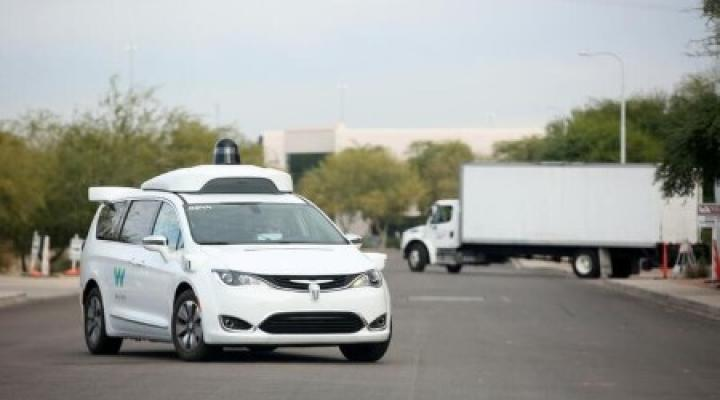
\includegraphics[width=.8\linewidth]{cars1.jpg}  
  \caption{Image 1. Displays a car in front and a truck further away on the right. This image is not from the KITTI data set.}
  \label{fig:sub-first}
\end{subfigure}
\begin{subfigure}{.5\textwidth}
  \centering
  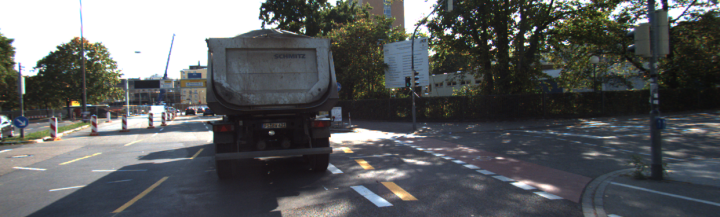
\includegraphics[width=.8\linewidth]{umm_000075.png}  
  \caption{Image 2. A truck in front, but open lanes on either side.}
  \label{fig:sub-second}
\end{subfigure}
\begin{subfigure}{.5\textwidth}
  \centering
  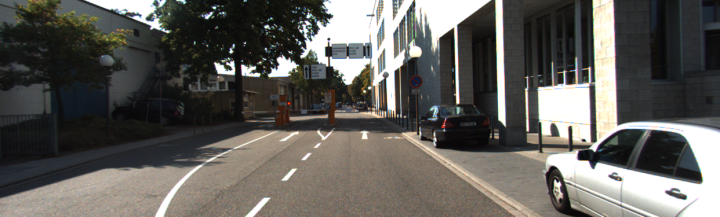
\includegraphics[width=.8\linewidth]{umm_000076.png}  
  \caption{Image 3. Open lanes in front and to the left, with cars parked on the right.}
  \label{fig:sub-third}
\end{subfigure}
\begin{subfigure}{.5\textwidth}
  \centering
  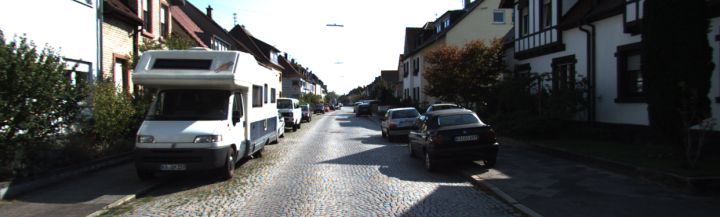
\includegraphics[width=.8\linewidth]{uu_000012.png}  
  \caption{Image 4. Open lane in front but vehicles parked on both sides.}
  \label{fig:sub-fourth}
\end{subfigure}
\caption{These four images depict different scenarios for street scenes. Images 2,3, and 4 were sourced from the KITTI data set.  }
\label{fig:fig}
\end{figure}

\subsection{Dense Captioning Results}
We applied our dense captioning model to and created a visualization of the regions for these four images. This creates a group of bounding boxes as well as a list of captions for each image. As stated in our methodology, the output for each caption has the information for the related boxes manually attached to it.

\begin{figure}[ht]
\begin{subfigure}{.5\textwidth}
  \centering
  \vspace*{3mm}
  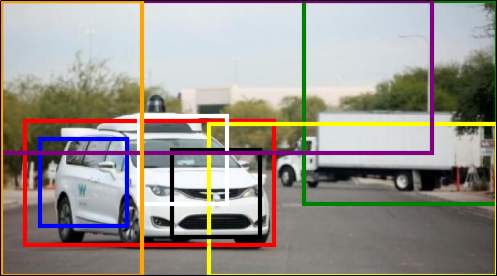
\includegraphics[width=.8\linewidth]{Figure_1.png}  
  \label{fig:sub-first}
\end{subfigure}
\begin{subfigure}{.5\textwidth}
  \centering
  \vspace*{3mm}
  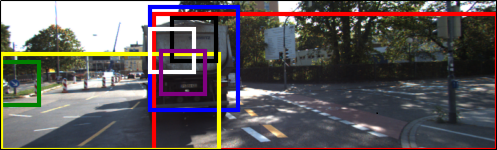
\includegraphics[width=.8\linewidth]{Figure_2.png}  
  \label{fig:sub-second}
\end{subfigure}
\begin{subfigure}{.5\textwidth}
  \centering
  \vspace*{3mm}
  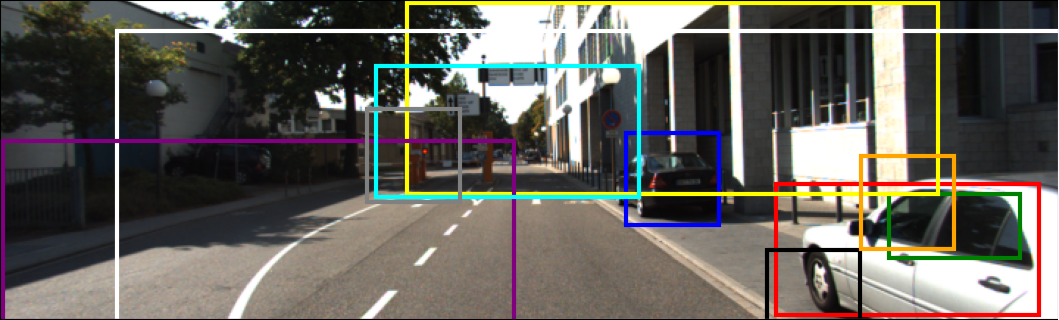
\includegraphics[width=.8\linewidth]{Figure_3.png}  
  \label{fig:sub-third}
\end{subfigure}
\begin{subfigure}{.5\textwidth}
  \centering
  \vspace*{3mm}
  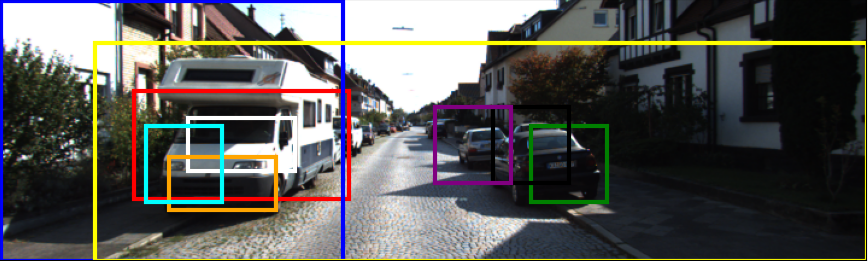
\includegraphics[width=.8\linewidth]{Figure_4.png}  
  \label{fig:sub-fourth}
\end{subfigure}
\caption{The visual results of the dense captioning on the images. Each bounding box represents a region in the results. }
\label{fig:fig}
\end{figure}

As seen in Figure 3, the bounding boxes capture significant objects in the road scene. Smaller boxes represent more constrained objects such as vehicles, windows, or wheels. Larger boxes represent loosely confined objects such as streets, roads, or the background. A bounding box may represent a single object or multiple different objects depending on the captions generated by the dense captioning model. When a logic predicate considers a box, it considers all objects that the box represents as well.

\subsection{Logic Query Results}
Table 1 shows the results of turning the data collected from the dense captioning model into predicates and running our logic base. True means that an action is determined to be safe, while false means the opposite. This output demonstrates that our logic model generates correct answers for the images given here. It is important to note that due to the differing dimensions between the images from KITTI and the image that wasn't, there were changes to the parameters of the bounding boxes that evaluated the parameters. Despite this, we still generate accurate results and further proves the strength of having an alterable and readable artificial intelligence as opposed to using machine learning techniques.

\begin{table}[htbp]
\caption{Safe Actions per Image}
\begin{center}
\begin{tabular}{|c|c|c|c|c|}
\hline
Action& Image 1& Image 2& Image 3& Image 4 \\
Go Forward& false& false& true& true \\
Change Lanes Left& false& true& true& false \\
Change Lanes Right& true& true& false& false \\
Brake& true& true& false& false \\
\hline
\end{tabular}
\end{center}
\end{table}

\subsection{Logic Query Results}
Following are the run times for the various sections of the experiment. The first two sections use machine learning while the third section uses only logic. The run time for the logic querying was consistently less than 1 ms.
\begin{table}[htbp]
\caption{Running Times in Seconds}
\begin{center}
\begin{tabular}{|c|c|c|c|c|}
\hline
Section& Image 1& Image 2& Image 3& Image 4 \\
Dense Captioning& 9.53& 9.53& 9.4& 9.54 \\
Predicate Generation& 3.82& 3.77& 3.91& 3.89 \\
Querying& 0& 0& 0& 0 \\
\hline
\end{tabular}
\end{center}
\end{table}
